
\section{Results}
\label{sec:results}

% Note that TeX has a mind of its own when it comes to placing images
% in documents - where a figure appears in the PDF document will often
% be quite different from where it appears in the source code. This is
% a feature, not a bug - it enables LaTeX to produce layouts that
% "flow" better. It only takes a few lines to insert a figure into
% your write-up - I recommend using PNG, JPG or PDF images
% (incidentally, programs like Excel and Matlab will allow you to save
% any plots or figures you generate in those formats). The \figure{}
% command is used to create a new figure.
\begin{figure}[htb]

  \centering  % centers the image in the column

  % replace the second argument below with your filename. I like to
  % place all my figures in a sub-directory to keep things organized
  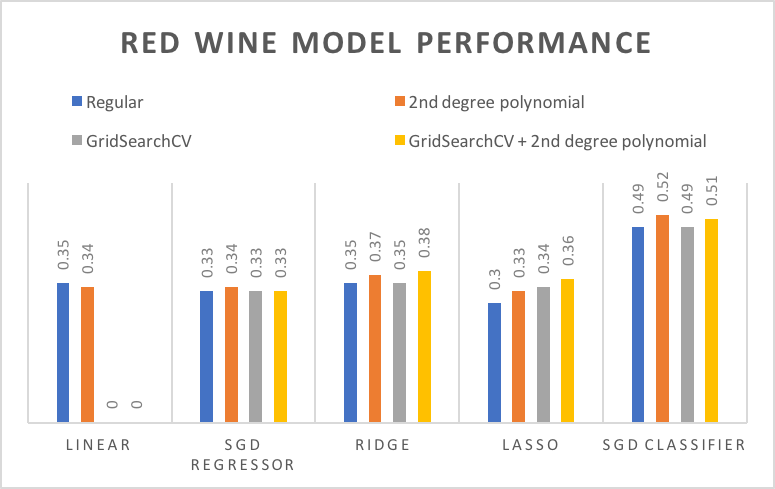
\includegraphics[width=0.47\textwidth]{redwine_score.png}

  % *Every* figure should have a descriptive caption.
  \caption{Visualization of red wine model performance at various experimental stages.}

  % The label is a handle you create so that you can refer to this
  % figure (using the \ref{} command) from other parts of your
  % document. LaTeX automatically renumbers figures and updates
  % references when you recompile, so you should do it this way rather
  % than hard-coding in references. Notice that I've also been
  % creating labels for the various sections in the document; I could
  % use \ref{} command to refer to those sections using their labels
  % too.
  \label{fig:tex}

  \end{figure}

  \begin{figure}[htb]

  \centering  % centers the image in the column

  % replace the second argument below with your filename. I like to
  % place all my figures in a sub-directory to keep things organized
  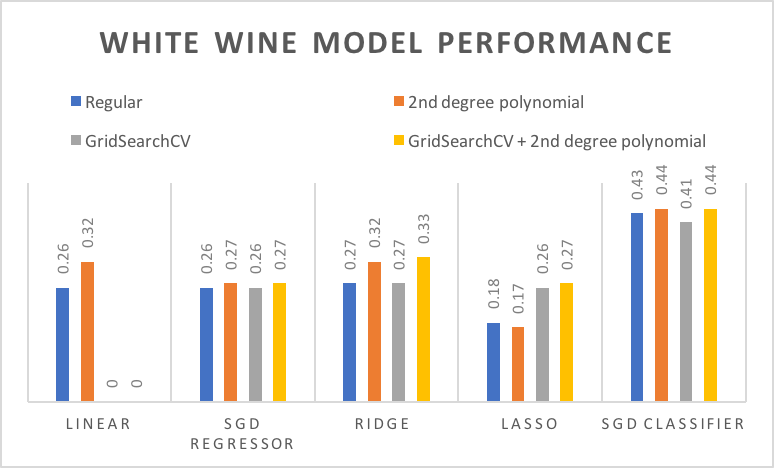
\includegraphics[width=0.47\textwidth]{whitewine_score.png}

  % *Every* figure should have a descriptive caption.
  \caption{Visualization of white wine model performance at various experimental stages.}

  % The label is a handle you create so that you can refer to this
  % figure (using the \ref{} command) from other parts of your
  % document. LaTeX automatically renumbers figures and updates
  % references when you recompile, so you should do it this way rather
  % than hard-coding in references. Notice that I've also been
  % creating labels for the various sections in the document; I could
  % use \ref{} command to refer to those sections using their labels
  % too.
  \label{fig:tex}

  \end{figure}
 

  
Our SGD Classifier model showed the best overall performance, for both red and white wines. However, since the SGD Classifier model wasn't explicitly discussed in class, we will focus more on the other models. Out of the other models, ridge regression proved to be the best model for both red and white wines. Running \texttt{GridSearchCV} improved the performance of all our models, except for \textt{SGDClassifier}. Using a second degree polynomial, on the other hand, was better all across the board, and increased the performance of all our models. A summary of our results can be seen in Figures 6 and 7.\\

Also, a quick note about feature selection. The reason we ended up using all the features is that for all five models, there were no significant improvements after we eliminated the least correlated two features. In addition, when we tried to eliminate more features, we noticed decreases in performance scores for all models. Thus, we decided that feature selection was not going to result in a significant performance improvement, and decided to use all the features.\\

Another interesting trend from our results is that all the models performed better for red wine than white wine. This isn't really what we expected, since we thought the large number of training examples in the white wine dataset would lead to a better model. A reason for this sub-par performance may have been because of an inherent disconnect between the features and the target for the white wine dataset. However, the main take-away from our experiments is that while implementing grid search helps in almost all cases, using a second degree polynomial helps even more. In most cases, using a second degree polynomial alone was roughly equivalent to using both \textt{GridSearchCV} and a second degree polynomial.

